\begin{figure}[H]
    \vspace{1em}
    \centering
    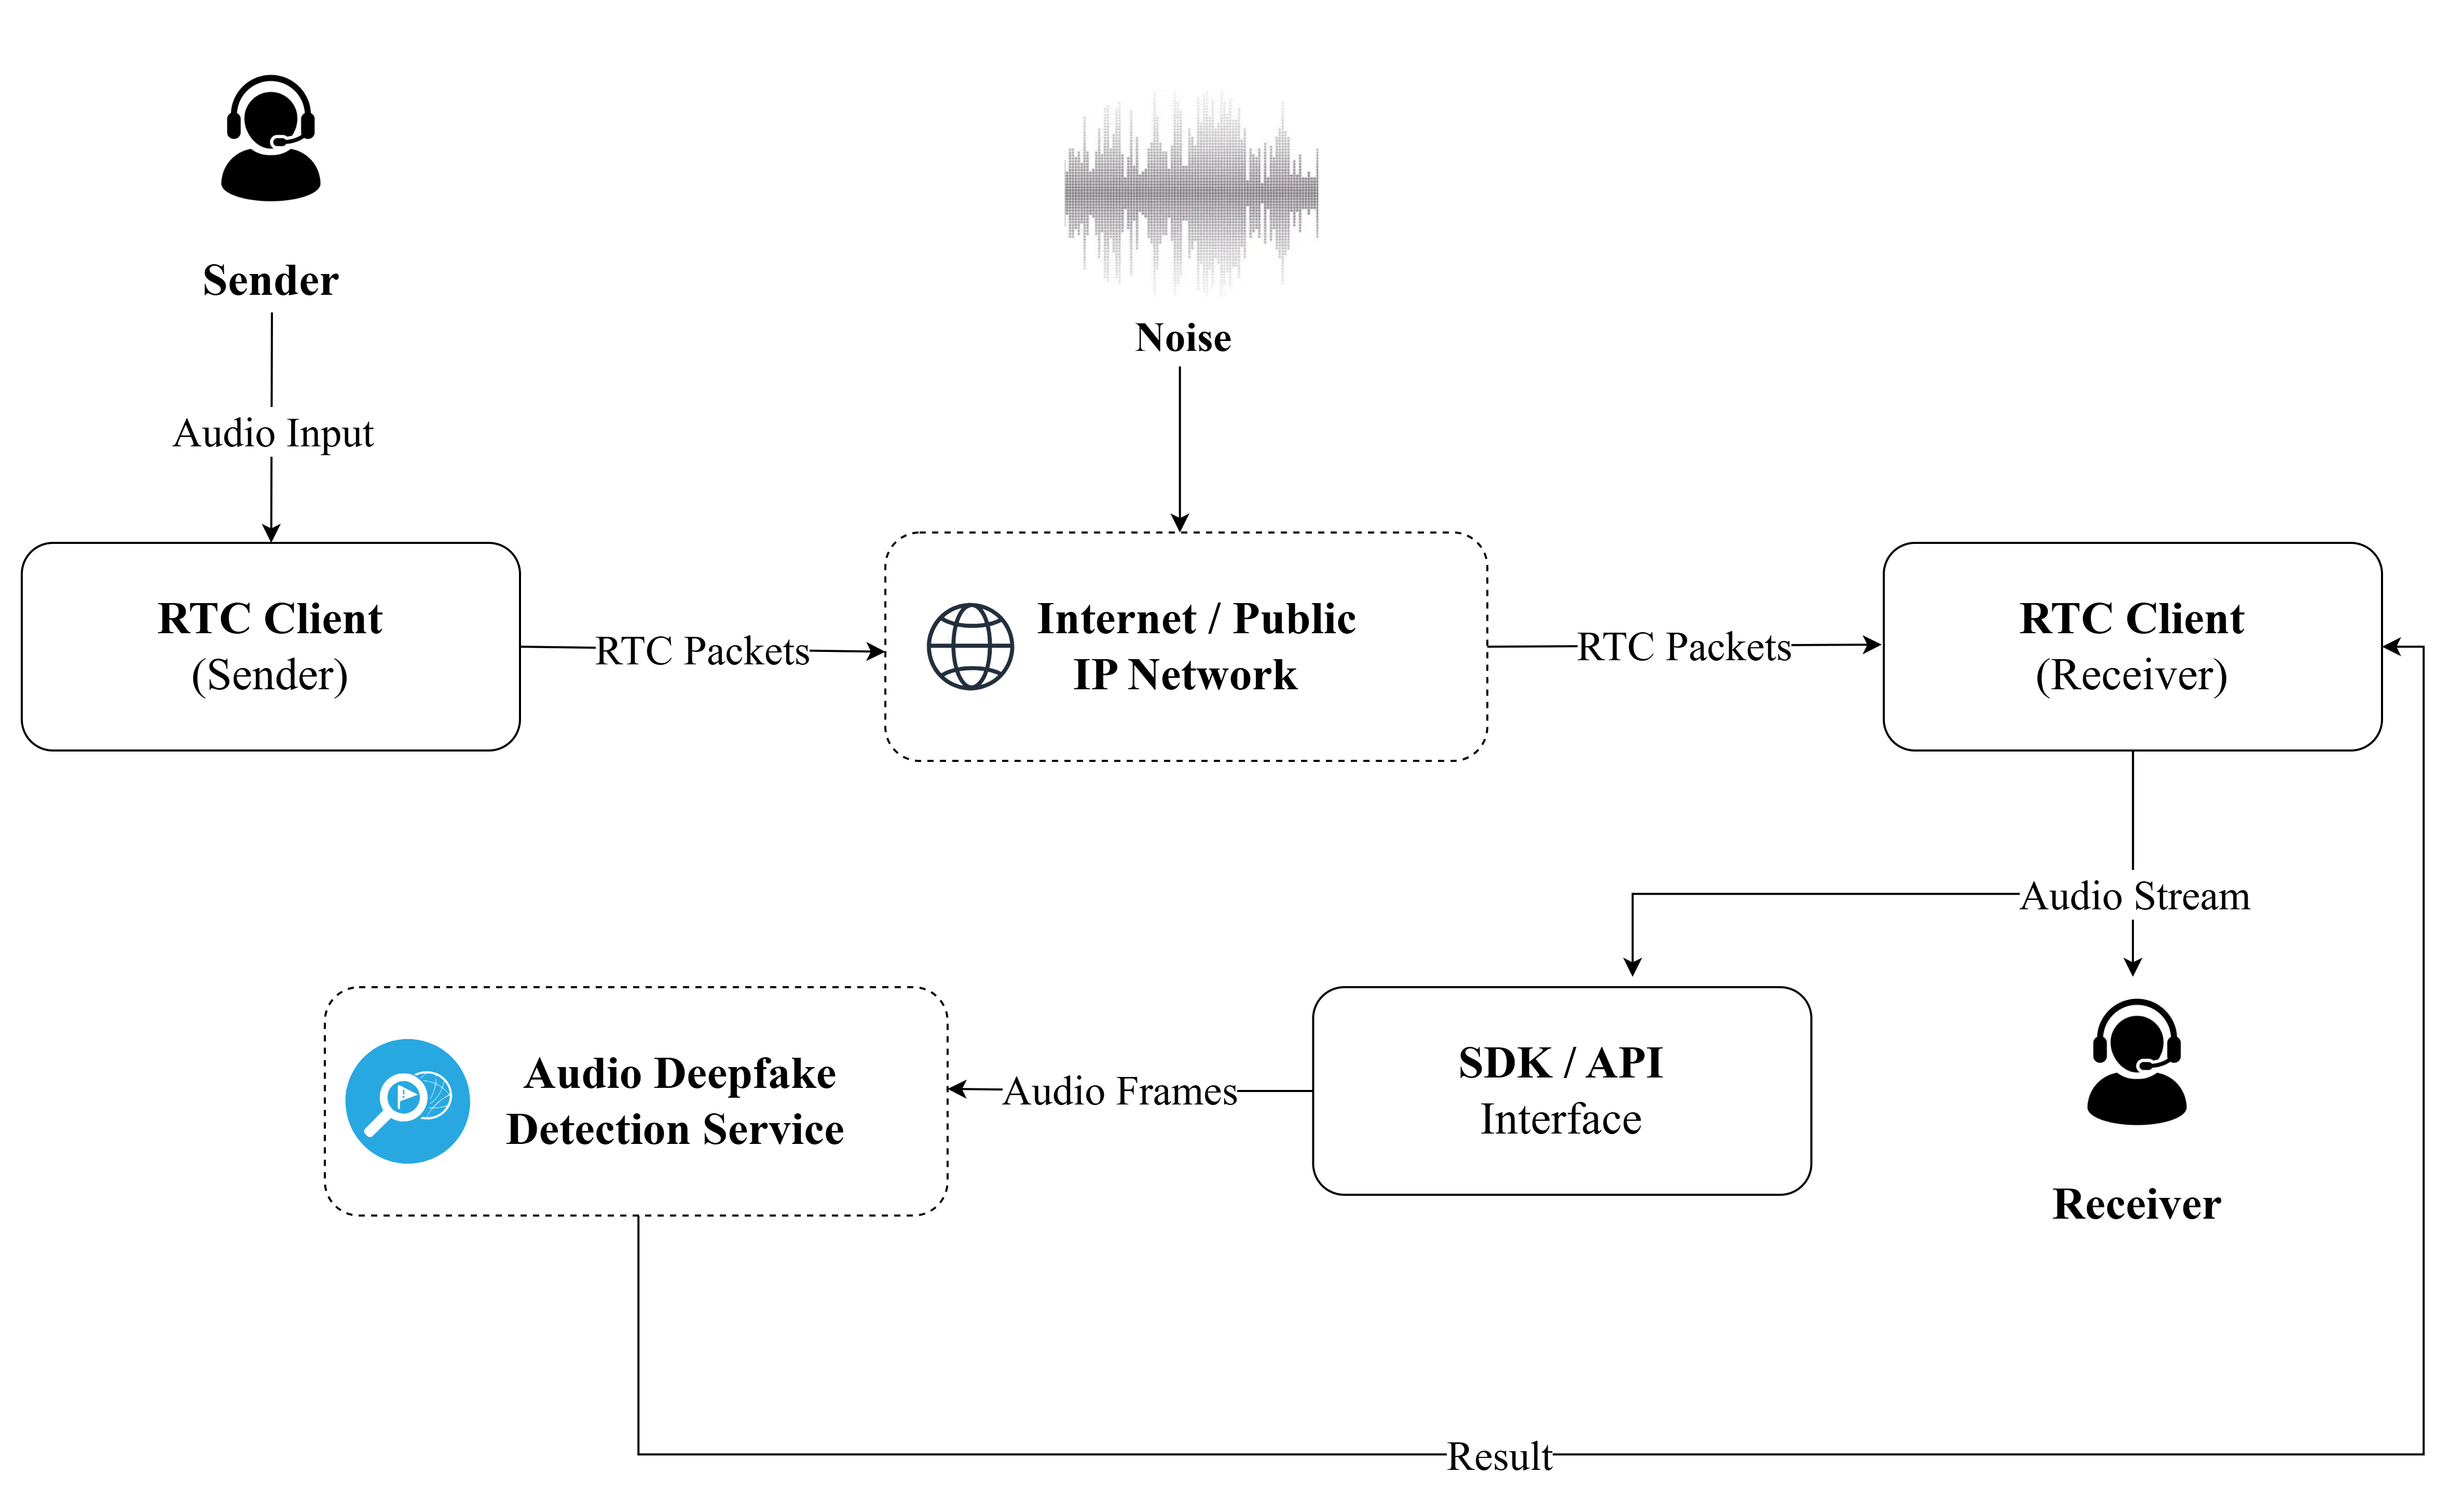
\includegraphics[width=1\textwidth]{images/methodology/system_block_diagram.png}
    \vspace{0.25cm}
    \caption{High-Level Design of the Proposed System}
    \label{fig:system_block_diagram}
\end{figure}

Figure~\ref{fig:system_block_diagram} presents the overall architecture of the proposed RTC-aware Audio Deepfake Detection (ADD) framework. The system is designed to detect synthetic speech during live communication sessions by operating on audio streams that have undergone realistic real-time communication (RTC) processing and transmission.

Unlike conventional deepfake detection approaches that operate on clean offline recordings, the proposed framework considers the complete communication pipeline through which speech is transmitted between users. During an RTC session, audio is captured at the sender side, compressed using communication codecs, packetized for network transport, transmitted across IP networks, reconstructed at the receiver side, and finally delivered for playback. Throughout this process, the speech signal experiences multiple transformations including codec compression, packet loss recovery, jitter buffering, and audio enhancement. These operations may alter or suppress artifacts commonly exploited by deepfake detection systems. Therefore, the proposed framework performs detection on the final reconstructed speech signal observed at the receiver side, closely reflecting practical deployment conditions.

The architecture consists of four major subsystems:
\vspace{-0.5cm}
\begin{enumerate}[label=\textbf{\arabic*.}]
    \item \textbf{Sender Side (RTC Client):} Captures speech from the speaker, performs audio preprocessing, codec encoding, and packetization before transmission.
    
    \item \textbf{Network Transmission Layer:} Transfers audio packets across IP-based networks where latency, jitter, packet loss, and routing variability may affect signal integrity.
    
    \item \textbf{Receiver Side (RTC Client):} Reconstructs the transmitted audio stream through packet reordering, jitter buffering, decoding, packet loss concealment, and audio enhancement operations.
    
    \item \textbf{Audio Deepfake Detection Service (ADD):} Operates as an external inference service that receives reconstructed audio from the receiver pipeline, extracts robust speech representations, performs deepfake classification, and generates spoofing risk assessments.
\end{enumerate}

The proposed system operates within a standard RTC communication scenario involving two communicating clients. When a call is established, speech captured by the sender-side RTC client is processed through the conventional transmission pipeline, including audio acquisition, preprocessing, encoding, packetization, encryption, and network transport. The transmitted packets traverse the communication network and are received by the receiver-side RTC client. The receiver reconstructs the speech signal through packet reordering, jitter buffering, packet loss concealment, decoding, and audio playback preparation.

Rather than modifying the communication process itself, the proposed framework introduces an Audio Deepfake Detection (ADD) service at the receiver side of the communication pipeline. After the speech signal has been reconstructed, a copy of the received audio stream is forwarded to the detection service for analysis. The ADD service extracts robust speech representations from the reconstructed audio and performs inference using a deep learning-based detection model. Based on the extracted features, the system generates a confidence score and a classification decision indicating whether the observed speech is real or synthetically generated.

The detection service is integrated through a non-intrusive plugin architecture, allowing it to operate independently from the RTC communication stack. A key design principle of the proposed framework is the separation between communication infrastructure and detection logic. Rather than modifying the underlying RTC protocols or media transport mechanisms, the system performs analysis on the reconstructed receiver-side audio stream. This approach preserves compatibility with existing RTC platforms while enabling the detection model to operate on speech signals that have already undergone realistic transmission, compression, buffering, and reconstruction processes.

Modeling the sender-side and receiver-side communication pipeline is important because audio transmitted through RTC systems undergoes multiple transformations before reaching the receiving user. These transformations introduce codec artifacts, quantization effects, packet loss recovery artifacts, buffering effects, and other network-induced distortions that may affect the discriminative characteristics used for deepfake detection. Consequently, the proposed system evaluates detection performance under realistic communication constraints rather than on pristine studio-quality recordings, thereby providing a more representative assessment of deployment-time performance.

The following sections describe each subsystem in detail, including the sender-side transmission pipeline, network transmission layer, receiver-side reconstruction process, and the proposed Audio Deepfake Detection service.
